% DO NOT EDIT THIS FILE
\documentclass[conference,harvard,brazil,english]{sbatex}
\usepackage[utf8]{inputenc} 
\usepackage{ae}
\usepackage{comment}
\usepackage{graphicx}
\usepackage{subfigure}


\begin{document} 

\title{A robotic system for \textit{in situ} hydropower turbine hard
coating} 

\author{Renan S. Freitas}{renan028@gmail.com} 
\address{Department of Electrical Engineering, COPPE
UFRJ, Rio de Janeiro, Brasil.}

\author[1]{Estevão Fróes}{ef.ferrao@mecanica.coppe.ufrj.br} 
\author[1]{Gabriel Alcantara C. S.}{alcantara@poli.ufrj.br}
\author[1]{Eduardo Elael M. S.}{elael2@gmail.com}
\author[1]{Ramon R. Costa}{ramonrcosta@gmail.com}
 
\twocolumn[ 
\maketitle
\selectlanguage{english}
\begin{abstract}
	Hard coating of hydropower turbine's blades increase power generation
	efficiency and system's life cycle. Currently, blade coating is an \textit{ex situ}
	process limited to unassembled turbines. EMMA is a robotic system for
	\textit{in situ} hard coating maintenance, overcoming the confined turbine's
	environment and constraints, and the process requirements. The proposed system
	is composed of modular and customized rails, a robotic manipulator, and sensors
	for control, localization and mapping. The simulations and field tests validate the concepts
	considered so far and rise several challenges for future works.
\end{abstract}
\keywords{Hard coating, manipulator, robotics, autonomous system, robot
calibration, rail system, hydropower}
\selectlanguage{brazil}
\begin{abstract}
	O processo de metalização das pás de turbinas hidrelétricas aumenta a
	eficiência da geração de energia, e sua vida útil. Atualmente, o
	revestimento das pás é um processo realizado fora do ambiente da turbina. EMMA
	é um sistema robótico para manutenção \textit{in situ} por metalização de pás
	de turbinas hidrelétricas, superando os desafios impostos pelo espaço
	confinado da turbina, seus requisitos e restrições do processo de metalização.
	O sistema é composto por trilhos modulares e customizados, um manipulador
	industrial robótico, e sensores para controle, mapeamento e localização. As simulações e testes de campo validam os
	conceitos considerados até agora e levantam novos desafios para trabalhos
	futuros.
\end{abstract}
\keywords{Metalização, manipulador robótico, robótica, sistema autônomo,
calibração, sistemas em trilhos, hidrelétrica} ] 

\selectlanguage{english}
 
\section{Introduction}
%RENAN - 1 pag

Hydropower has an important share in the global electricity production, and
will continue to be a major source of renewable
power-generation\footnote{International Energy Agency (2010), http://www.iea.org/.}% \cite{iea}.
. In hydropower generating plants, the average maintenance cost is 2\% of the
investment cost per kW, and typically, the large mechanical
components, as turbines, must be maintained and replaced every 25 years.
The cavitation and abrasion phenomena on the turbine's blades have become a
concern, as the erosion can lead to water flow instability, excessive
vibrations and turbine efficiency reduction \cite{goldemberg2007energia}. Hard
coating techniques by thermal aspersion are used to greatly increase the life
cycle of runner's blades~\cite{krella2011new}.

In the specific case of Brazil, hydropower is the largest
power-generation source. To support future economic growth, Brazil has
invested in additional large hydroelectric facilities, for instance, the
14~GW Belo Monte along the Xingu River\footnote{Energy
Information Administration (2014), https://www.eia.gov/.}%~\cite{eia}
, and Jirau dam (Fig.~\ref{fig::jirau_turb}) along the Madeira river. At the
latter, the high concentration of suspended particles carried by the river intensifies the abrasion phenomena, thus
regular maintenance is needed. Currently, blade coating maintenance in these
large facilities is performed before turbine assembling by a large-sized
robotic manipulator, i.e., it is an \textit{ex situ} process. 

Repair maintenance, as grinding and welding, can be done manually in the
turbine's environment, but the hard coating procedure requires a robotic system
due to high precision, speed, and the usage of hazardous substances.
There are several difficulties encountered when attempting to robotize
\textit{in situ} maintenance, as accessibility, system placement and
calibration. A few robotic systems have been investigated to perform \textit{in
situ} repair of turbine runners, as it could greatly improve efficiency and
safety, while decreasing operational and logistical
costs~\cite{hazel2012field}, but none has been used for the hard coating operation. Some examples found in the literature are:

\begin{figure}[h!]
\centering
	\includegraphics[width=.8\columnwidth]{figs/intro/jirau_turb.JPG} 
	\caption{Jirau's hydropower turbine.}
	\label{fig::jirau_turb}
\end{figure}

\begin{itemize}
\item The Roboturb~\cite{roboturb} and the Scompi~\cite{scompi} are robotic
systems to perform erosion inspection and welding on damaged runner's blades.
They move on a flexible rail, which may be shaped and then fixed to the blade
surface.

\item \textit{The Climber}\footnote{International Climbing Machines (2013),
http://www.icm.cc/.} %~\cite{icm}
 is an intervention robot for wind and hydroelectric turbines, to perform
coating removal, surface cleaning and coating application. It is a climbing
robot with pneumatic adhesion and locomotion by tracks.
\end{itemize}

In this paper, we present a general overview of a robotic system called EMMA,
and a detailed description of the mechanics, the manipulator, and
calibration. The system performs \textit{in situ} hydropower
runner's blade hard coating, and it is composed of an industrial manipulator
that moves on customized rails, a 3D laser scanner for mapping, and
sensors for positioning feedback.
\begin{comment}
The system operate in a confined space, move
on a sloping and slippery environment through a rail, identify the runner's
blades, calibrate its position, generate the path planning and perform the hard
coating. 


This text is organized as follows: a general overview of the robot and its main
challenges are presented in Section \ref{sec:general_overview}, detailed
descriptions of the embedded electronics, the vehicle support system, power
supply system, and software architecture are taken in
Sections \ref{sec:electronics_overview}, \ref{sec:powersupply_overview}, and
\ref{sec:software} respectively.
In Section \ref{sec:results}, preliminary results are shown, and concluding
remarks are drawn in Section \ref{sec:conclusions}.
\end{comment}
\section{The hard coating process and the project requirements}\label{hvof}

Hydropower runner's blades are typically eroded by cavitation and abrasion
phenomena, resulting in hydraulic profile deformation, thus efficiency
reduction. The High Velocity Oxygen Fuel (HVOF) coating is a preventive
solution for erosion, and creates a lamellar structure. 

The HVOF is a 2000~hp power process which consists of spraying coating particles
by an 8~kg spray gun, through a flame with mixed gases. To achieve the best
coating layer, the spray gun should be at a fixed 210~mm to 240~mm distance, and
$90^\circ \pm 30^\circ$ angle, in respect to the metallic surface plane of the
blade; and the gun should move at 40~m/min speed along the path
\cite{li2002effect}.  Besides, for a regular coating cover, the trajectory is
3~mm spaced horizontal lines crossing the blade's surface (coating step), which
requires great positional accuracy of the robot.
The common solution which meets the requirements for \textit{ex situ} HVOF
coating is a robotic manipulator with a blade-sized workspace in a fixed
position.

\section{The problem}\label{problem}

The problem is to design a robotic system for \textit{in situ} hard coating of
hydropower runner's blades. Accessibility is a major problem: the robot must be
brought to the turbine through a 800~mm diameter hatch; and it must operate in
the confined, curved, slippery and harsh environment of the turbine. Besides, there are
several control and calibration problems, as robot kinematics and
dynamics, trajectory planning, and robot localization.

The mechanical challenges are robot locomotion, base stiffness, and fixation.
The robot should be transported and positioned in turbine's environment, as the
access is generally far from the runner's blade.
The stiffness is required for the hard coating process, since vibrations can be
propagated from manipulator's base to the end-effector with high
amplitudes, compromising the coating quality.

Regarding calibration, the relative position between the manipulator and the
blade is not fixed. The system calibration consists in the identification of
the manipulator and blade, and their pose estimation in respect to the turbine
interior. Due to the environment's light conditions, 3D laser sensing
technology should be used to map the topography of the blade, the
environment, and the robotic system. 

Large-sized manipulators are not suitable for \textit{in situ} operations, due
to the accessibility and confined space; and conventional compact manipulators
do not have the required work envelope or payload for the task. Therefore,
customized or mid-sized manipulators should be investigated by kinematics and
dynamics simulations. Besides, the robot control strategy comprises the
blade modeling, the automatically trajectory generation,
and the robot position and velocity control.


\begin{comment}

A bulb type turbine has the following points of interest for solution
development: 1) the variable pitch propeller, or Kaplan \textbf{blades}; 2) the
variable pitch guide vanes, or \textbf{wicket gates}; 3) the \textbf{runner
area}; 4) the \textbf{draft tube}; and 5) an access for regular
maintenance, or \textbf{hatch}. The Jirau's turbine is the case study of EMMA,
thus a 3D CAD model was built with SolidWorks\raisebox{1ex}{\textregistered}
for simulation and solution analysis (Fig.~\ref{fig::ambiente3d}).

\begin{figure}[h!]
\centering
	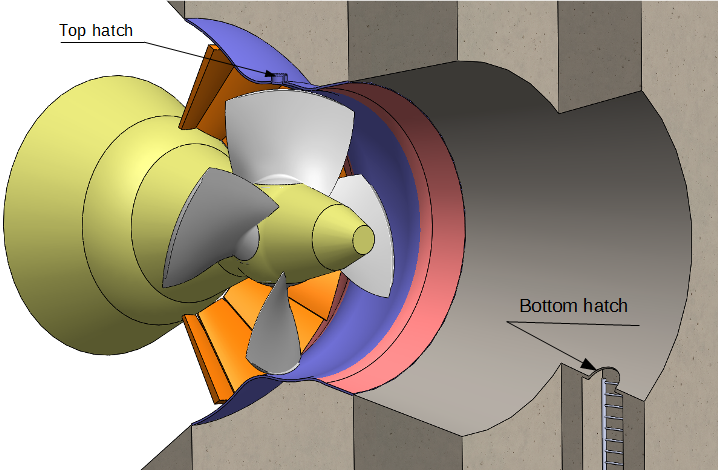
\includegraphics[width=\columnwidth]{figs/problem/ambiente_3d.PNG} 
	\caption{Jirau's hydropower turbine in a 3D CAD model.}
	\label{fig::ambiente3d}
\end{figure}

\end{comment}
\section{Solution}\label{solution}

%2.5 pages
%Renan: Solucao-Intro
%Renan: Solucao-Manipulator
%Estevão: Solucao-Rails (Renan revision)
%Estevão/Renan: Solucao-Shutter
%TODO Gabriel: Solucao-Calibration

EMMA robotic technology is described in this section. The following system's
elements will be presented: the robotic manipulator; the customized modular
base; and the robot calibration. 

\begin{comment}
The Jirau's t urbine is the case study of
EMMA, thus a 3D CAD model was built with
SolidWorks\raisebox{1ex}{\textregistered} for simulation and solution analysis.

Its hardware is composed
of a mid-sized robotic manipulator, a customized modular rail base, and
vision-based sensors. As the manipulator cannot fully cover the blade's surface in a fixed
position, and the robot locomotion is complex in the turbine's environment, a
customized rail is designed to provide extra degrees of freedom (DOF) to the
system. EMMA aims to be a generic solution to large bulb type turbines, being
modular, and versatile. 
\end{comment}


\subsection{Robotic Manipulator}\label{manipulator}
The HVOF coating requirements and environment constraints demand a mid-sized
robotic manipulator (Sec.~\ref{hvof}), as a large-sized one would not
be able to move inside the confined space, and a small-sized manipulator would not
have the required payload and speed. In EMMA's project, the
robotic manipulator will be responsible for the coating application, precision, and tool handling.

A market survey is conducted to determine the most suitable robotic
manipulator for the application. Overall simu\-lations and analysis were performed using the OpenRave \cite{diankov2008openrave},
an environment for simulating motion planning algorithms for robotics. There are
several tools for dynamics simulation of robots: Gazebo, V-Rep,
Webots, and others% \cite{ivaldi2014tools}
. OpenRave stands out for having the following features: integral design for
real-time control and execution monitoring; core functionality for kinematics operations and
physics simulations; a network protocol allowing interpreted scripting
languages; built-in core tools and plugins for manipulation planning and
sensing systems.

The simulations involve runner's blade discretization, base
position computations for full cover, and robotic manipulator's kinematics
and dynamics. 

The blade's surface discretization is an uniform sampling to
determine where to the coating directions should be. The current ; standard plugins that allow testing of different planning
algorithms and sensing systemsapproach is to
take the bounding box of the blade and sample its surface uniformly. Once the
surface of the box is sampled, the intersection of the blade and a ray
originating from each point going inward is taken. The normal of the blade's
surface from each of these intersection points is taken to be the coating
direction. As an uniform sampling of the box does not mean an uniform sampling
of the blade, the box is oversampled and a 50~mm filter is applied, by a multidimensional search key with k-d tree.
The samples are translated 230~mm in respect with their normal vectors,
and collision checks with the environment are made. 

Base position computations are to uniformly sample the turbine's
confined space and to calculate the required robotic manipulator's base
positions to process all the samples (blade discretization),  considering angle
and distance tolerances. It is a brute force search: for each position, inverse
kinematics are computed to determine the robotic manipulator's joint parameters that provide
the desired positions and orientations of the end-effector.

The kinematic approach described above is not enough to ensure that the robot
will reach the samples. Maximum accelerations, decelerations,
torques, and jacobian singularities should be investigated and compared to the robotic
manipulator's specifications. The Newton-Euler method
\cite{sciavicco2000differential} was adopted for torque computation: $\tau =
M(q)\alpha + C(q,\omega)\omega + G(q)$, where $\tau$ is the joints' torques,
$M$ is the matrix of links' masses and moments of inertia, $\alpha$ is the
joints' accelerations, $q$ is the joints' angles, $\omega$ is the joints'
velocities, $C$ is the Coriolis matrix, and $G$ is the gravity vector.

In the dynamic approach, $M$ was estimated by the robotic manipulator's CAD
model. The angular accelerations are derived by differential kinematics:
$\alpha=J^+(a-\omega^TH\omega)$, where $H$ is the Hessian matrix
\cite{hourtash2005kinematic}, $a=\ddot{X}$ is the linear accelerations, and $J$
is the Jacobian matrix. Therefore, torques can be analytically estimated with
the inverse dynamics in OpenRave. 

% The typical path of HVOF coating is a zigzagging trajectory,
% i.e., it is a deceleration and acceleration process with direction changes. As
% the \textit{ex situ} solution uses a large-sized robotic manipulator, the
% end-effector's direction changes occur outside the blade's range, complying the
% speed requirement in the blade's range. However, while deceleration or
% acceleration, coating material is wasted to the environment or, most commonly,
% to a shadow plate.
% 
% The mid-sized robot for \textit{in situ} operation makes this strategy
% impossible, as, at some base positions, the robot will always be in the blade's
% range. The proposed solution modifies the original circuit of the gases that
% carry the coating particles to a new 2-way controlled circuit, in which there is
% a directional valve that changes the flow path from the thermal spray gun to return to tank
% circuit. The directional valve is autonomously actuated accordingly to the robotic
% manipulator's trajectory, i.e., the valve will ``shut'' while end-effector
% changes its direction. Therefore, the solution provides coating material
% savings, as the non-used particles are stored for future usage, and the hard
% coating speed requirement is met.

% \begin{figure}[h!]
%    \centering
%    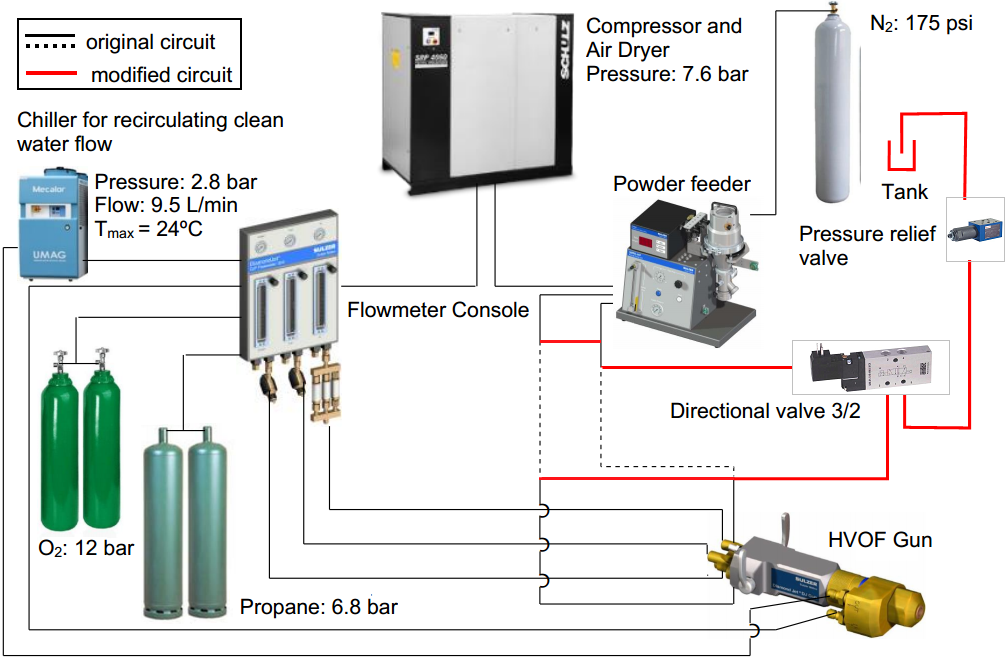
\includegraphics[width=0.9\columnwidth]{figs/mecanica/Circuito_HVOF_mod_en.PNG}
%    \caption{Simplified view of HVOF circuit with shutter}
%    \label{fig::circuito_hvof}
% \end{figure}

 

\subsection{Base}
% 0.75 pages

EMMA's base comprises two rails, forming two prismatic joints (P). The
first, or primary rail, is parallel to the turbine axis, and it is responsible
for the transportation of the robotic manipulator from hatch to blade. The
secondary rail is parallel to the blade's surface, and it is assembled from the
first rail by a rotational joint (R). 

\begin{figure}
	\centering
	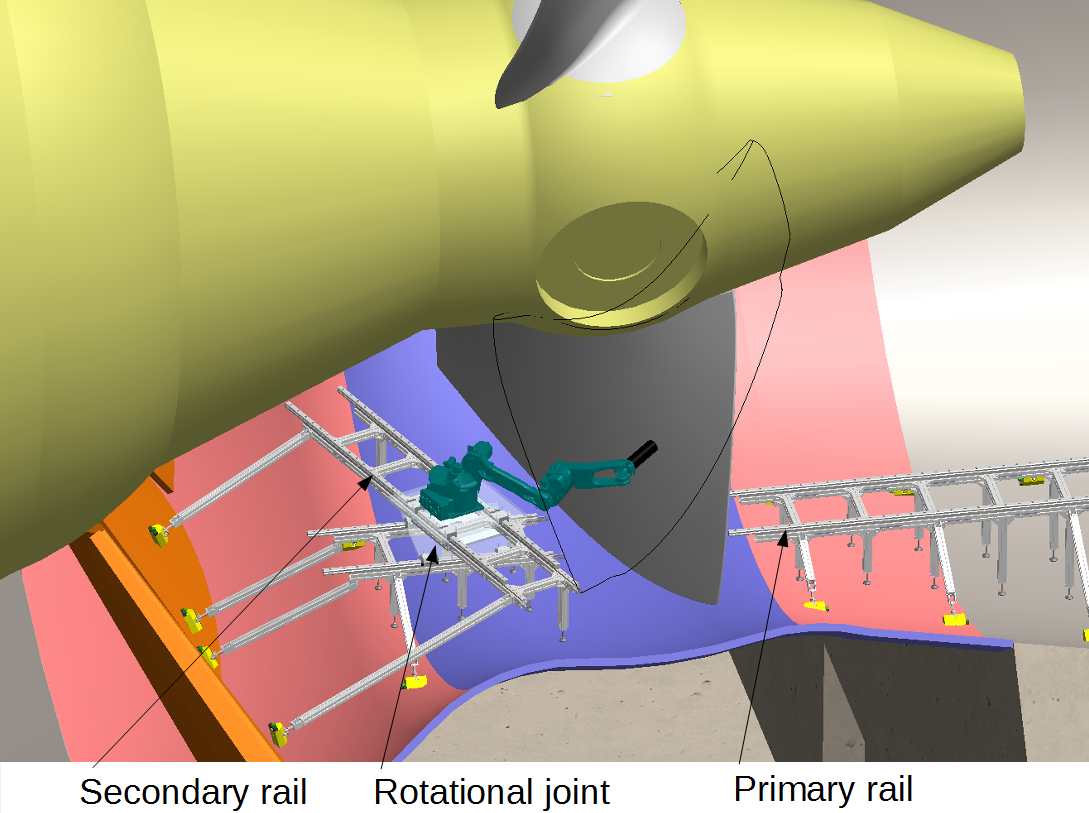
\includegraphics[width=.9\columnwidth]{figs/mecanica/EMMA_Base_Secundaria_02.PNG}
    \caption{Customized base: primary and secondary rails.}
    \label{fig:base}
\end{figure}

The hatch and turbine' space can limit the size of the rail in terms of weight
and geometry, thus a modular concept was design, such that the small modular parts can be easily and
manually assembled inside the turbine. The base is a modular two parallel
profiled rail with a four carriage setup%  \cite{SKF_2013}
. In this
configuration, the reaction moments of the base are cancelled by a force couple provided by each couple of
carriages. The commercial modules are aluminum structures for corrosion resistance,
lightweight, geometric flexibility, and modularity, as it is possible to
increase/decrease the rail length/width/height by changing few parts or adding
anchor arms.

The resulting base is a slender and lightweight frame, such that a careful
analysis is necessary to evaluate the structural integrity and rigidity in
respect to the dynamic loads of the robotic manipulator. A Finite Element
Analysis (FEA) was performed to study the stresses, strains and resultant forces
along the structure. FEA is also used to size the frame components, such as
the profile's size, and to size the anchors, its directions, and attachment to
provide the greater base's rigidity. The rigidity is a major concern, it is
required for the hard coating process, since a non-rigid base propagates
vibrations to the robotic manipulator's end-effector with high amplitudes, which
may compromise coating quality.

The draft tube and runner area are conical shape structures, curved and
sloped. The environment modification, as wielding and drilling, should be
avoided, thus properly fixing the base on the ground is a major challenge in
EMMA project. The draft tube is composed of a ferromagnetic steel material,
hence magnetic fixtures is suitable for base attachment. 

\begin{comment}
Common magnetic fixture products are temporary magnetic equipments used to hoist
and transport materials in an industrial plant. In EMMA, it is used to attach
and anchor the rail's modules to the ground.
\end{comment}

\subsection{Calibration}
 
In hard coating \textit{in situ} operations, the relative position between the
manipulator and the blade is not fixed. The system calibration consists in the
indentification of the manipulator and blade, and their pose estimation in
respect to the turbine interior. Due to the light conditions inside the
hydraulic circuit a 3D laser scanner is used to gather 
information of the environment, including the  manipulator and base.

\begin{comment}
The calibration process was divided in two different approach depending on the
element to be localized and its caracteristics. The possibility to attach or
install markers in known positions dictated the strategies to be chosen,
therefore the calibration is separeted in the pose estimation of the robot and
of the blade, as follows.
\end{comment}
   
The attachment of markers on the robotic manipulator can be performed with high
precision and repeatability, thus reflective spheres were chosen as reference
points in the process of robot localization. These spheres are identified inside
the point cloud by the 3D Hough Transform method \cite{camurri20143d}. The 3D
Hough Transform, as the 2D Hough Transform, is the search of an object on the
(discretized) parametric space. A sphere has four parameters: three for the
position of its center, and one for its radius. For each point on the point
cloud, it is assigned a collection of voxels on the discretized parametric
space, corresponding to the possible spheres passing through that point. As in
a voting process, the voxels with the greatest number of points assigned to
define the parameters of the most probable spheres. There might be computational
issues depending on the size of the parameter space, but it can be mitigated by
exploiting previous knowledge regarding the expected radius and viable region
for the robot inside the enviroment.

Fixing any marker on the blade would require its own calibration to ensure a
consistent reference point, thus the pose estimation of the blade must rely only
on the intrinsec properties of its surface geometry. The information must be extracted from
the point cloud (the scene) provided by the 3D laser sensor and
compared to a reference model previously stored. The characteristics of the point clouds are represented
by local descriptors, i.e., each interest point on the blade is associated
with a piece of information about its local neighborhood. Given the
sets of features from the model and the scence,  it is possible to determine the
correspondence between their descriptors. If enough correspondences are found
in the scene, above a threshold, the blade is identified and the position can be
determined \cite{Tombari2010a}.

As the blade is a large and smooth surface, the neighborhood of each point may
introduce similiar information, creating ambiguous descriptors that degrade the
matching perfomance, thus it is fundamental to wisely pick the interest points.
The ambiguous descriptors provide information about perpendicular translation to
the supporting plane, and the two rotations associated with it, thus no
information about the other DOFs, making the alignment to ``slide'' from the
correct transformation. Therefore, the interest points were sampled to
diversify the normal vectors' directions \cite{Rusinkiewicz2001}, allowing to
reduction of the number of samples to have a descriptor associated, when
compared to a uniform sampling, and maintaning the computational cost low.


Once the descriptors were estimated, the correspondences are determined if the
euclidean distance between a descriptor in the scene and in the model is lower
than a threshold. Each correspondence vote for a specific pose and scale factor in the
Hough space. After an instance of the model is found, it is performed the 
Iterative Closest Point (ICP) matching with the full resolution point clouds to
realize a fine alignment and compensate any discrepancy introduced by the
sampling. With the position of the blade and the manipulator in respect to a
common coordinate system, i.e., the origin of the laser sensor, it is possible
to determine the transformation between them and this information can be fed to
the trajectory and coverage algorithms.




\section{Results}

% 1 page
%Renan: Results-Intro
%TODO Gabriel: Results-Calibration
%Estevão: Results-Mecanica
%Renan: Results-Control

% Intro

Simulations and experimental tests were performed to verify the proposed
concepts. The following results were divided according to the EMMA system's
elements introduced in Sec.~\ref{solution}. 


\subsection{Robotic manipulator analysis}\label{sec::man_analysis}

As stated in Subsec.~\ref{manipulator}, simulations for the robotic
manipulator were implemented with OpenRave, and consist of the following steps:
blade's surface discretization; coating strategy; coating segmentation
(partitioning) and base positions computation; kinematics, dynamics and
manipulability.

The blade's surface discretization is an uniform sampling of the blade to
determine where to the coating directions should be. However, sampling the
actual geometric surface can lead to unwanted results due to possible
concavities. A simpler approach is to take the bounding box of the blade and
sample its surface uniformly (\textit{axis-aligned bounding box}). Once the
surface of the box is sampled, the intersection of the blade and a ray
originating from each point going inward is taken. The normal of the blade's
surface from each of these intersection points is taken to be the coating
direction. As an uniform sampling of the box does not mean an uniform sampling
of the blade, the box is oversampled and a 50~mm filter is applied to the
resulting sampling of the blade, by a multidimensional search key with k-d tree.
The result is an uniformely sampled blade, and the samples are spaced
50~mm from each other. These samples are translated 230~mm in respect with their
normal vectors, collision checks with the environment are made, and the
feasible samples are named \textit{coating samples}.
Fig.~\ref{fig:discretization} shows blade's discretization and the
\textit{coating samples}. 

\begin{figure}
	\centering
	\subfigure{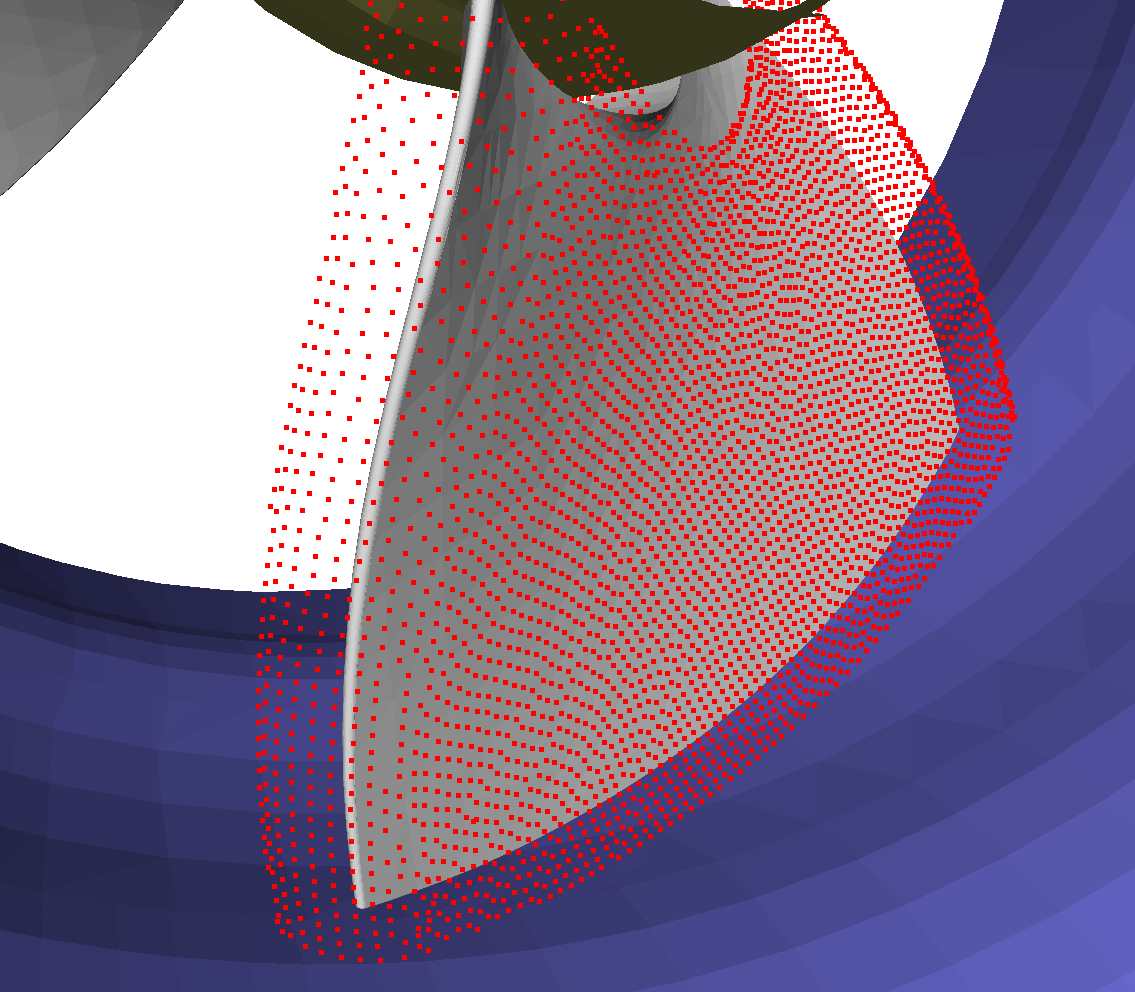
\includegraphics[width=0.47\columnwidth]{figs/results//blade_grid1.png}}\quad
	\subfigure{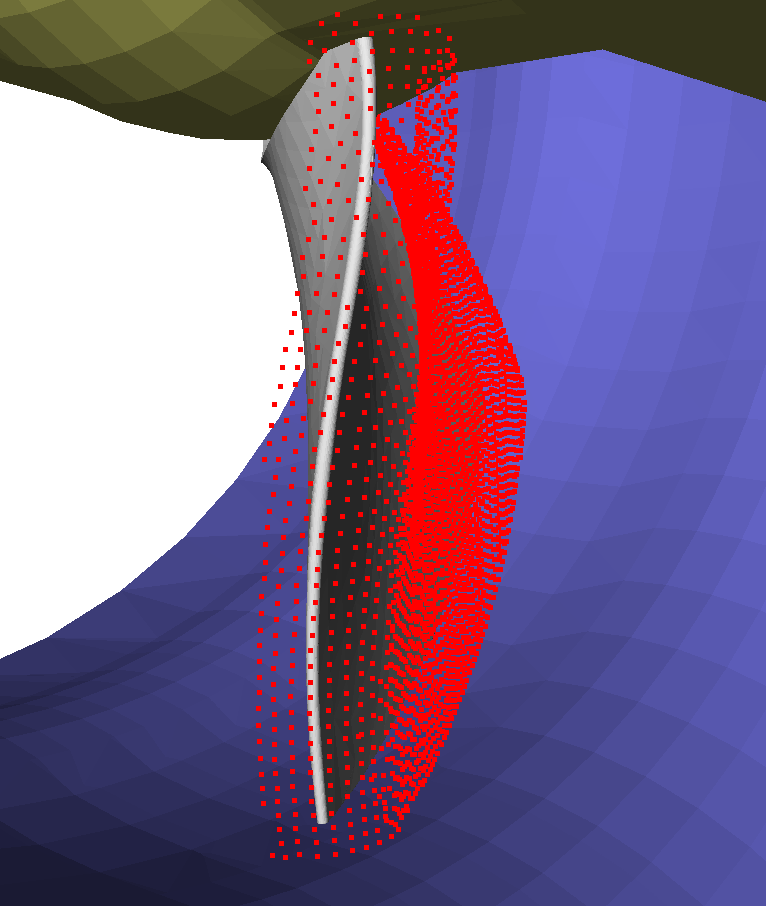
\includegraphics[width=0.47\columnwidth]{figs/results//blade_grid2.png}}
    \label{fig:discretization}
    \caption{Blade discretization and \textit{coating samples} in red}
\end{figure}

The coating segmentation and base positions computation is to calculate the
required robotic manipulator's base positions to process all the \textit{coating
samples} with angle and distance tolerances. It is a brute force search, in
which the positions are uniformly sampled in the turbine's confined space. For
each position, inverse kinematics (IKFast) are computed to determine the
robotic manipulator's joint parameters that provide the desired positions and
orientations of the end-effector. Fig.~\ref{fig:coating} shows examples of the
algorithm, where black dots are coated points and blue dots are coated points
with angle tolerance. At the end of the Alg.~\ref{alg:strategy}, the reachable
samples are in the Matrix~\ref{algvar:reachable}, which relates coating samples
with base positions, thus it is possible to create a coating strategy and to
select the simplest base positions. The result is the minimum required
positions for the robotic manipulator's base.

\begin{figure}
	\centering
	\subfigure{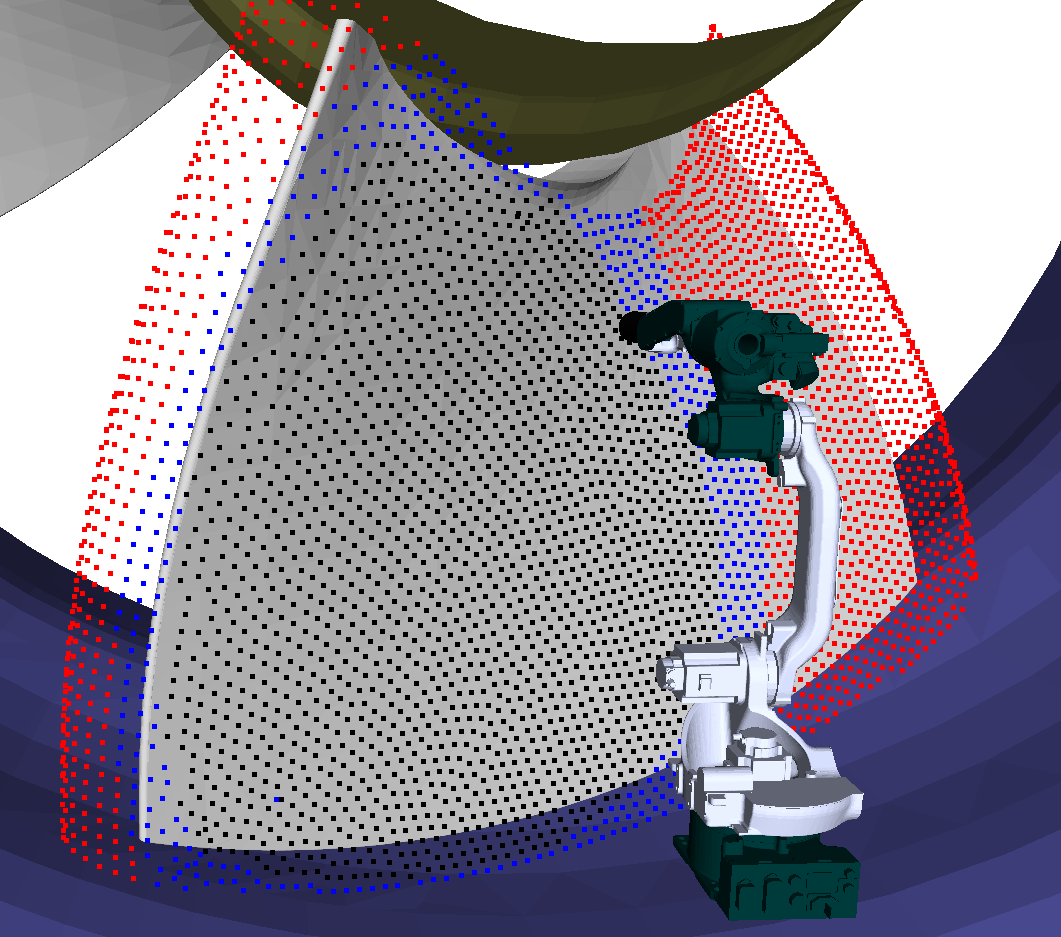
\includegraphics[width=0.47\columnwidth]{figs/results/mh12_coating1.png}}\quad
	\subfigure{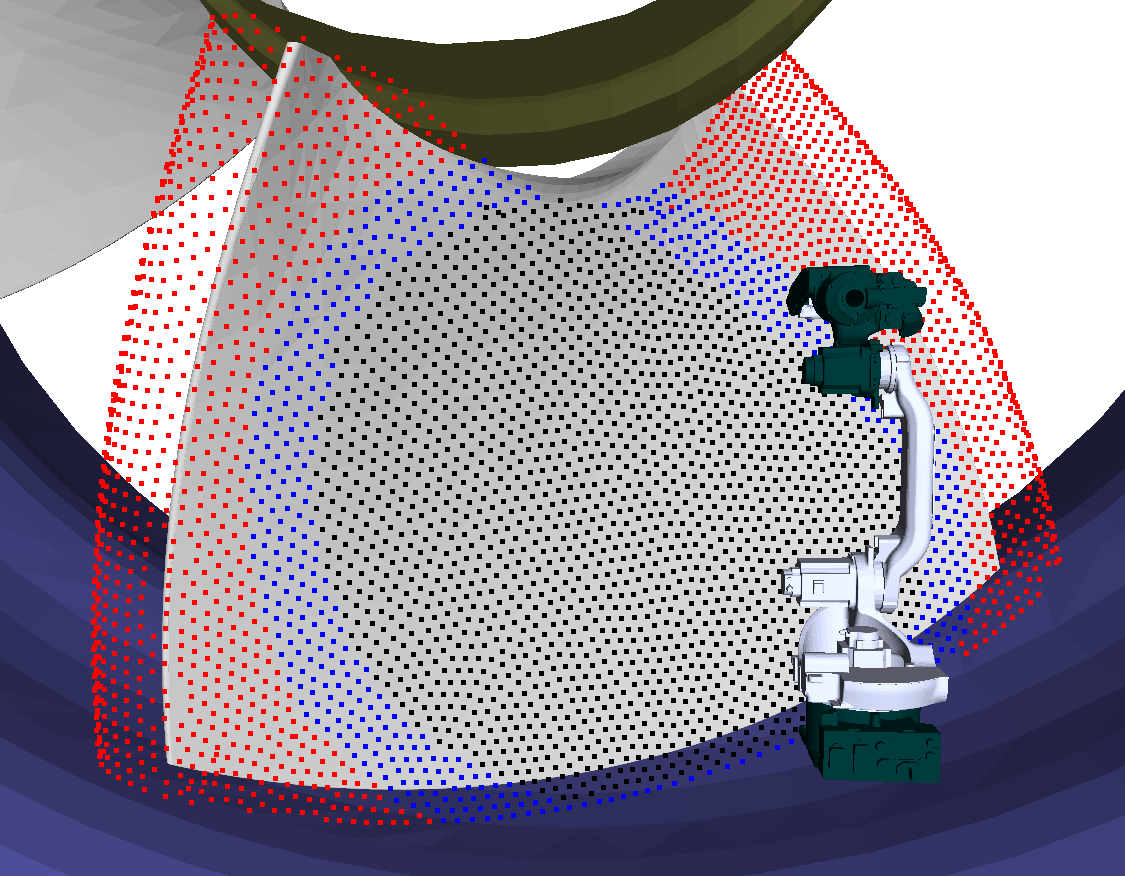
\includegraphics[width=0.47\columnwidth]{figs/results/mh12_coating2.png}}
    \caption{Robotic manipulator coating samples.}
     \label{fig:coating}
\end{figure}

\begin{algorithm}
\caption{Coating strategy}
\label{alg:strategy}
\begin{algorithmic}[1]
\ForAll{Base positions} 
		\ForAll{\textit{Coating samples}}
			\State Joints = IKFast(sample)
			\If{not Joints} 
				\State Joints = IKFast(sample,tol)
			\EndIf
			\If{Joints} 
				\State $\textrm{Reachable}[\textrm{pos}] += [\textrm{sample}]$
				\label{algvar:reachable}
			\EndIf
		\EndFor
\EndFor
\end{algorithmic}
\end{algorithm}

The kinematic approach described above is not enough to ensure that the robot
will reach the \textit{coating samples}. Maximum accelerations, decelerations,
torques, and jacobian singularities should be investigated and compared to the robotic
manipulator's specifications. The Newton-Euler method
\cite{sciavicco2000differential} was adopted for torque computation: $\tau =
M(q)\alpha + C(q,\omega)\omega + G(q)$, where $\tau$ is the joints' torques,
$M$ is the matrix of links' masses and moments of inertia, $\alpha$ is the
joints' accelerations, $q$ is the joints' angles, $\omega$ is the joints'
velocities, $C$ is the Coriolis matrix, and $G$ is the gravity vector.

In the dynamic approach, $M$ was estimated by the robotic manipulator's CAD
model. The angular accelerations are derived by differential kinematics:
$\alpha=J^+(a-\omega^TH\omega)$, where $H$ is the Hessian matrix
\cite{hourtash2005kinematic}, $a=\ddot{X}$ is the linear accelerations, and $J$
is the Jacobian matrix. Therefore, torques can be analytically estimated with
the inverse dynamics in OpenRave. Comparing estimated torques with the technical
specifications, dynamics simulations's results showed that the robotic
manipulator should be placed at, at least, 1400~mm distance from the blade's
surface. Placing the robot nearer would enhance the robotic manipulator's
workspace, but it would increase the torques also, above the technical
specifications. Fig.~\ref{fig:torques} shows joints' torques for blades's
\textit{coating samples} in a color gradient way, where red dots represents
small magnitudes and blue dots large magnitudes. The Fig.~\ref{fig:torques} is
an example of the robotic manipulator in a close range, 900~mm distance from the
blade.

\begin{figure}
	\centering
	\includegraphics[width=.5\columnwidth]{figs/results/manipulability_colorgradient.png}
    \caption{Robotic manipulator joints' torques in color gradient.}
    \label{fig:torques}
\end{figure}

\subsection{Base analysis}

The FEA analysis of the base verifies the Von Mises stress and displacements
along the structure's slender members. The stress analysis determines the
integrity of the base due to the maximum loads of the robotic manipulator. The
displacements determine if the structure provides a rigid base for the robotic
manipulator. According to the hard coating requirements, displacements of the
order of millimeters are not even allowable in the elastic region of the
material.
%TODO Estevão: big displacements é generico. 

%TODO Estevão: falar o programa utilizado para a análise, numero de elementos
% finitos e parametros necessarios para reproduçao da analise

%TODO Estevão: corrigir formato compilado das referencias estilo techreport

The FEA software used to solve the analysis was the Nastran
In-CAD$^{\mbox{\small\textregistered}}$ integrated to the
SolidWorks'$^{\mbox{\small\textregistered}}$ interface. The elements are bar
Line Elements (1-D) and a mesh of global size 25~mm. The material properties are for 
the EN AW-6060~\cite{DIN_2007} as the material used for the aluminum profile
structure and are in accordance to the table~\ref{tab::prop_material}. The
boundary conditions are the 3 translational constraints for the anchor arms and
a vertical constraint to the feet. The rotational joint is modeled as a rigid
conector between the rails, the same way as the robot's base with respect to the
second rail. The maximum dynamic forces and moments \cite{MH12_manual} are
applied as static loads, to the point that represents the origin of the robot's base. 

\begin{table} [h!]
\centering
\begin{tabular}{|l|l|l|}
\hline
\textbf{Properties}   & \textbf{Value}   & \textbf{Units}	  \\ \hline
Density			       & $2700$           & kg/$m^3$          \\ \hline
Young Modulus		   & $70,0$           & GPa               \\ \hline
Shear Modulus		   & $26,1$           & GPa               \\ \hline
Poisson's Ratio		   & $0,34$           &                   \\ \hline
Yield Strength  	   & $200$            & MPa               \\ \hline
\end{tabular}
\caption{EN AW-6060 Properties}
\label{tab::prop_material}
\end{table}

The maximum Von Mises stress was 5.78~MPa, which gives a factor of safety of
34.6. It was found for a particular case where the robotic manipulator is in
the secondary rail, 800~mm from the rotational joint. The displacement of the
structure causes a maximum translation of 0.47~mm and a angular deflection of
$0.0149^{\circ}$ in respect to robotic manipulator base's coordinate system. 
%TODO Estevão: figura!

%TODO Estevão: Testes in situ com a base magnética


\subsection{Calibration analysis}

Field tests are very complex due to the logistics and the availability of a dry
hydropower turbine, thus simulated data were analyzed, which can be consistent
and can represent effectively the actual operation scenario. In calibration
analysis, turbine's environment and the robotic manipulator were simulated with
the toolbox Blensor \cite{Gschwandtner11b}. The blade's model, however, was
acquired in a field test by a 3D laser scanner for a better representantion of
the actual hidraulic profile.

The laser sensor was modeled following manufacturer's technical
specifications, and different scenes were generated for several sensor's
positions. The algorithm is able to localize the blade in respect to the
sensor's coordinate system, even in occlusion by the presence of the robotic
manipulator. In Fig.~\ref{fig:calibration}, the left yellow blade is the
reference model, the red blade is the object to be found, and green lines
represent the matching features between the model and the scene.

\begin{figure}
	\centering
	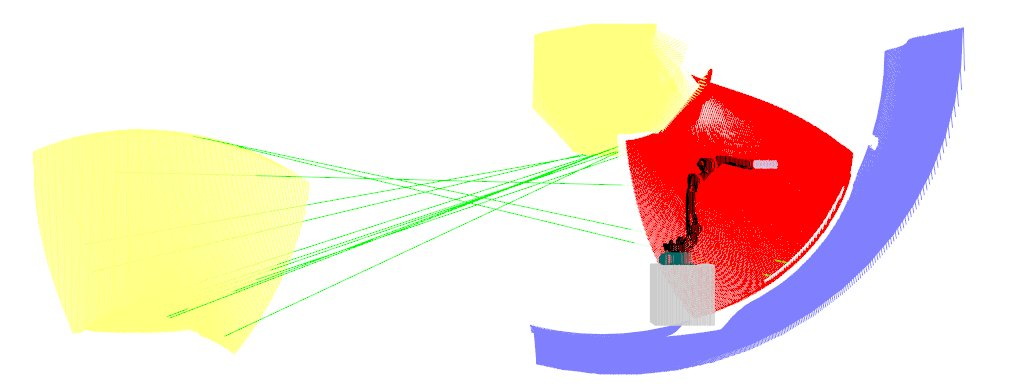
\includegraphics[width=.95\columnwidth]{figs/results/sim_mh12_sp}
    \caption{Robotic manipulator joints' torques in color gradient.}
    \label{fig:calibration}
\end{figure}
\section{Conclusion and future work}

% 0.5 pages

In this paper, we presented the concept solution and general overview of EMMA
project.

%TODO Elael: Conclusion and Future Work
\section*{Acknowledgements}
We gratefully acknowledge the financial support of Energia Sustentável do
Brasil and the ANEEL R\&D program (contract COPPETEC/UFRJ JIRAU 09/15
6631-0003/2015).


\bibliography{main} 
\end{document}